\chapter{Tests}

\section{Funktionale Tests}\label{sec:tests-functional}

\todo{Write}

\clearpage
\section{Load Tests}\label{sec:tests-load}
Zur Umsetzung des Load Testings wurde Apache JMeter eingesetzt.\\

Während funktionale Tests die Korrektheit der Implementierung prüfen,
evaluieren Load Tests die Performance des Systems unter hoher Last,
beispielsweise bei vielen nebenläufigen Zugriffen.
Es gibt zahlreiche Gründe eine Anwendung Load Tests zu unterziehen.
Diese sind unter anderem:

\begin{itemize}
    \item Messung der Systemperformance
    \item Identifikation von Bottlenecks
    \item Skalierbarkeit des Systems prüfen
    \item Entdeckung von Race Conditions
\end{itemize}

\subsection{Starten von JMeter}

JMeter kann im GUI- oder CLI-Modus gestartet werden.
Der GUI-Modus wird zum Erstellen und Debuggen von Tests eingesetzt,
welche anschließend im CLI-Modus ausgeführt werden können.

JMeter startet standardmäßig im GUI-Modus.
Um Tests im CLI-Modus auszuführen, kann folgender Befehl eingesetzt werden.

\begin{lstlisting}[caption=Beispielkonfiguration des CLI-Modus]
    jmeter -n -t testplan/TestPlan.jmx -l "results/result.jtl" -j "logs/logs.log" -eof reports/
\end{lstlisting}

Die eingesetzten Optionen haben folgende Bedeutung:

\begin{itemize}
    \item \texttt{-n} - CLI-Modus
    \item \texttt{-t} - Pfad zum Testplan
    \item \texttt{-l} - Pfad zur Testlogdatei (Testergebnisse)
    \item \texttt{-j} - Pfad zur Jmeterlogdatei (Informationen über Testausführung und aufgetretene Fehler)
    \item \texttt{-e} - Report generieren
    \item \texttt{-o} - Pfad für Reportdateien
    \item \texttt{-f} - Alte Ergebnisse und Reports löschen
\end{itemize}

\subsection{Erstellung von Testplänen}

Tests werden in Form eines Testplans geschrieben.
Ein Testplan ist ein Baum, der Elemente aus verschiedenen Kategorien enthalten kann (siehe \url{https://jmeter.apache.org/usermanual/test_plan.html}).

\begin{itemize}
    \item Thread Groups kontrollieren wie oft Sampler ausgeführt werden, insbesondere wie viele Anfragen nebenläufig stattfinden.
    \item Logic Controller beeinflussen die Ausführungsreihenfolge der Sampler.
    \item Sampler enthalten die auszuführenden Tests, z.B. HTTP-Anfragen.
    \item Listener speichern die Ergebnisse eines Samplers und können diese im GUI-Modus grafisch aufbereiten.
    \item Configuration Elements stellen Daten für Tests zur Verfügung, unter anderem durch Definition von Konstanten,
          Erzeugung zufälliger Werte oder Einlesen externen Dateien.
\end{itemize}

%\vspace{2em}

Die Elemente können auf unterschiedliche Weise verschachtelt werden, gängig ist dabei folgende Reihenfolge:

\begin{itemize}
    \item Der Testplan enthält \texttt{Thread Groups}, wobei jeder Thread einer Gruppe einen User darstellt.
    \item \texttt{Thread Groups} enthalten \texttt{Sampler}, welche von jedem Thread der Gruppe von oben nach unten ausgeführt werden.
    \item \texttt{Samplers} enthalten (einen) Listener, welcher die Ergebnisse aufzeichnet und im GUI-Modus visualisieren kann.
    \item \texttt{Configuration Elements} werden nach Bedarf als Kinder von \texttt{Thread Groups}, 
    \texttt{Samplers} oder dem Wurzelelement des Testplans definiert.   
\end{itemize}

\begin{figure}[h]
    \centering
    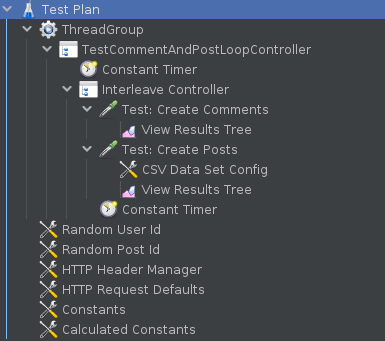
\includegraphics[width=0.65\linewidth]{Graphics/Testplan.png}
    \caption{Beispiel eines Testplans}
\end{figure}

\subsection{Report Dashboard}\label{sec:Dashboard}

JMeter kann die erfassten Leistungsparameter in einem HTML-Dashboard zusammenfassen. 
Dieses besteht aus verschiedenen Graphen, welche etwa Antwortzeiten und Datendurchsatz über den Verlauf des Tests darstellen.
Um einen Report zu generieren, muss die Option \texttt{-e} benutzt werden.
Das Dashboard ist direkt ohne weitere Konfiguration benutzbar und sollte für die meisten Projekte ausreichend sein.
Nur in fortgeschritteneren Anwenungsfällen, etwa zur automatischen Auswertung, 
ist die Verwendung von Listenern mit eigenen Result-Dateien notwendig.

JMeter unterstützt Anpassungen an der Graphgenerierung, etwa das Einstellen der zeitlichen Auflösung.
Weiterhin können eigene Graphen hinzugefügt werden. 
Siehe hierzu \url{https://jmeter.apache.org/usermanual/generating-dashboard.html}.

Ein Beispielreport befindet sich im Ordner \texttt{jmeter/ReportBeispiel}.



\subsection{Verwendung von Variablen und Scripting}

JMeter ermöglicht die Definition von Variablen und Skripten, um Tests besser wart- und anpassbar zu machen.

Zur Definition von Variablen kann etwa das Configuration Element \texttt{User Defined Variables} eingesetzt werden.
In diesem Element definierte Konstanten können grundsätzlich mit der Syntax \lstinline|${Variablenname}| referenziert werden,
allerdings wird diese Syntax nicht überall unterstützt.
So funktioniert dies etwa im Körper einer HTTP Request oder zur Angabe der Wiederholungen einer Threadgroup,
nicht aber zur Angabe von Dateipfaden für Sampler.

JMeter unterstützt mehrere Skriptinterpreter (Beanshell, Groovy, Javascript, Jexl). 
Die Dokumentation empfiehlt die Verwendung von Groovy oder Jexl3.
Skripte können statt Literalen zur Definition verschiedener Parameter des Testplans eingesetzt werden.
Die Syntax zur Ausführung von Skripten folgt diesem Schema: \lstinline|${__interpreter(script)}|.

Wird die Verwendung einer Variable mittels \lstinline|${Variablenname}| nicht direkt unterstützt,
kann der Wert der Variable oftmals durch ein Skript ausgelesen werden.
Hierzu kann darin die Funktion \lstinline{vars.get("Variablenname")} benutzt werden.
Leider funktioniert auch dieser Ansatz nicht in allen Fällen.

Scripting ermöglicht die Berechnung von Konstanten in Abhängigkeit von anderen Konstanten.
Die abhängige Konstante muss in einem eigenen \texttt{User Defined Variables}-Element definiert werden.
Dieses muss sich im Baum unter dem ursprünglichen Konfigurationselement befinden.
Wird die Konstante im gleichen Element oder einem im Baum höherstehenden Element definiert,
scheitert die Auflösung der abhängigen Variable und sie wird als leerer String behandelt.

\begin{lstlisting}[caption=Beispiel eines Groovy-Skripts]
    ${__groovy(
        vars.get("UserCount").toInteger() 
        * vars.get("PostsPerUserCount").toInteger()
    )}
    \end{lstlisting}

Um Fehler beim Einsatz von Variablen zu untersuchen,
kann der Sampler \texttt{Debug Sampler} eingesetzt werden.
Dieser wertet bei Ausführung alle verfügbaren Variablen aus, sodass deren Werte überprüft werden können.
Die Werte sind im GUI-Modus unter \texttt{Response Data} des zum Sampler hinzugefügten Listener einsehbar.

\subsection{Relative Pfade}

JMeter bietet keine vollständige Unterstützung für relative Pfade.

Die Angabe relativer Pfade ist im GUI-Modus nicht möglich.
Ersetzt man im durch den GUI-Modus erzeugten Testplan, einer XML-Datei, absolute durch relative Pfade,
so werden diese im CLI-Modus korrekt aufgelöst.
Öffnet man den manipulierten Testplan erneut im GUI-Modus,
kann JMeter die relative Pfade jedoch nicht auflösen.

Um trotzdem absolute Pfade zu vermeiden, 
kann ein Basispfad als Variable definiert werden.
Pfade werden dann als Konkatenation dieser Variable und des gewünschten relativen Pfades definiert.
Der Basispfad kann als Literal oder durch ein Skript definiert werden.

\begin{lstlisting}[caption=Ermitteln des Working Directory\protect\footnotemark]
    ${__BeanShell(
        import org.apache.jmeter.services.FileServer; 
        FileServer.getFileServer().getBaseDir();
    )}
    ${__BeanShell(File.separator,)}
\end{lstlisting}
\footnotetext{Quelle:\url{https://stackoverflow.com/questions/11268015}}

\section{Continuous Integration}

\textit{Die \ac{CI}-Definitionen liegen im Verzeichnis} \texttt{.github/workflows}.\\

Da wir nun alle Tests geschrieben haben, wollen wir dass diese automatisiert ausgeführt werden und Reports geben zum aktuellen Stand der Implementierung im Repository. Dazu benutzen wir \textbf{Github Actions}. Diese konfigurieren wir so, dass alle Tests (siehe \ref{sec:tests-functional} und \ref{sec:tests-load}) automatisch bei einem Git-Push auf das Repository ausgeführt werden.

Sollten Tests fehlschlagen wird dies automatisch durch diese Pipeline festgestellt und benachrichtigt den Autor des Commits.
Des Weiteren generiert der Workflow für die Load-Tests einen HTML-Report mit Performance-Indikatoren und Graphen (siehe \ref{sec:Dashboard}).
